\subsection{Unilateral spring oscillator}
\label{sec:oscillator}
We reproduce the unit-mass oscillator of Junca and Rousselet \citep[Sec.~2]{junca2009}. Its displacement obeys $\ddot u+\omega_0^2 u+\varepsilon[u]_+=0$, with $u(0)=a_0>0$ and $\dot u(0)=0$. We use the normalizations $\omega_0=1$ and $a_0=1$ and select $\varepsilon/\omega_0^2=0.1$ for the parameterized model. The oscillator spends $\pi/\sqrt{\omega_0^2+\varepsilon}$ time units in contact and $\pi/\omega_0$ detached per period. Matching the two harmonic solutions at $u=0$ gives the displacement and contact force $\varepsilon[u]_+$ throughout the run.

We integrate 50 periods with the HHT solver and evaluate the scalar spring law directly. Linear interpolation of the numerical displacement at neighboring steps gives the times of contact onset and release. Each run reproduces all 100 transitions. Table~\ref{tab:oscillator} shows the refinement results. At the finest step, the largest timing error over the run is $2.09\times10^{-4}$ time units. The maximum errors in the duration of complete contact and detached intervals are $2.15\times10^{-6}$ and $2.05\times10^{-6}$ time units, respectively. Figure~\ref{fig:oscillator} shows the displacement and the accumulated timing error. This case tests integration through repeated changes of contact state with an exact force callback.

\begin{table}[pos=!htbp]
\centering\small
\caption{Errors over 50 periods of the published unilateral spring model. RMS displacement and force errors and the maximum onset or release timing error use the normalized units of the reproduction.}
\label{tab:oscillator}
\begin{tabular}{lrrr}\toprule
Nominal step & RMS displacement error & RMS force error & Max. timing error \\\midrule
0.0100 & $1.44\times10^{-3}$ & $1.01\times10^{-4}$ & $3.35\times10^{-3}$ \\
0.0050 & $3.60\times10^{-4}$ & $2.52\times10^{-5}$ & $8.37\times10^{-4}$ \\
0.0025 & $9.01\times10^{-5}$ & $6.29\times10^{-6}$ & $2.09\times10^{-4}$ \\
\bottomrule\end{tabular}
\end{table}

\begin{figure}[pos=!htbp]
\centering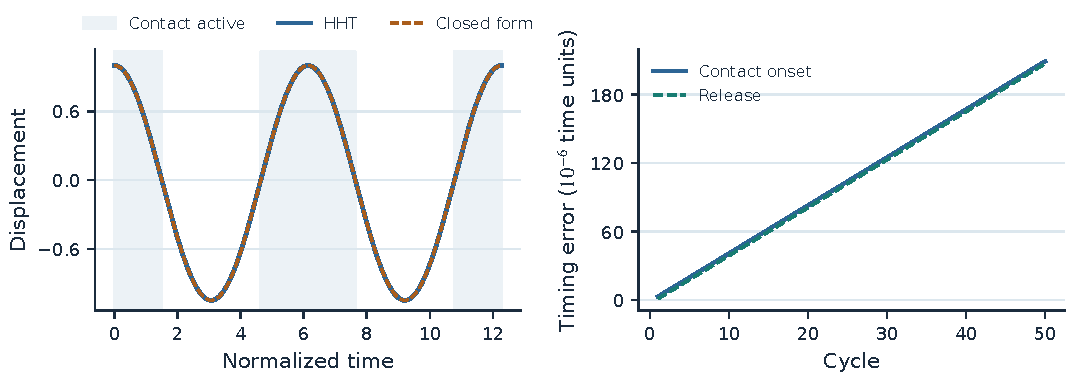
\includegraphics[width=.92\linewidth]{unilateral-response.pdf}
\caption{Unilateral oscillator with the finest HHT step. The first two periods show the motion and intervals of active contact. The onset and release timing errors are shown for all 50 periods.}
\label{fig:oscillator}
\end{figure}

\subsection{Constant-breadth cam and translating flat follower}
\label{sec:constant-breadth}
We reconstruct the Type I cam in Dhande and Rajaram's Example~1 \citep{dhande1984} from the six circular arcs of their Table~1. We use $a=6$, $b=5$, $c=7$, $d=2.5$, and $x_0=y_0=0$ in their length units. The cam rotates at $1$ rad/s between two parallel follower faces. Its constant breadth is $9$ length units. The guide and the opposing faces prescribe the follower translation. The reference comprises their displacement, velocity and acceleration equations over one complete revolution (Eqs.~(8), (10), and (12) and Table~2).

We rotate the reconstructed B-rep and obtain displacement from its supporting position along the follower translation axis. Position evaluation uses the CAD profile and its oriented extrema. Five-point finite differences at a spacing of $0.05^\circ$ yield velocity and acceleration. At the six arc junctions the acceleration changes discontinuously, so we report derivative errors at the 7,175 positions with stencils wholly inside an arc's contact interval. The maximum absolute CAD reconstruction errors are $2.66\times10^{-15}$ in displacement, $4.50\times10^{-12}$ in velocity and $1.31\times10^{-8}$ in acceleration, in the corresponding length and second units. Figure~\ref{fig:constant-breadth} shows the reconstructed motion and reference.

On the original $1^\circ$ sample grid we also import the CAD profile's extruded arc faces from STEP and use our bounded distance query to obtain a follower position interval at each pose. The 361 intervals, including both endpoints, contain the published position. The widest interval is $9.99\times10^{-5}$ length units and the maximum midpoint error is $4.91\times10^{-5}$ length units. This case verifies contact geometry and prescribed kinematics across all six profile sections.

\resultfigure{constant-breadth}{Reconstructed constant-breadth cam at $90^\circ$ between two translating flat faces, with an enlarged view of the contact on the right face. CAD kinematics and published solutions use the original length units and time in seconds. Acceleration curves are broken at the arc junctions.}{fig:constant-breadth}
